%%
%% Copyright 2007, 2008, 2009 Elsevier Ltd
%%
%% This file is part of the 'Elsarticle Bundle'.
%% ---------------------------------------------
%%
%% It may be distributed under the conditions of the LaTeX Project Public
%% License, either version 1.2 of this license or (at your option) any
%% later version.  The latest version of this license is in
%%    http://www.latex-project.org/lppl.txt
%% and version 1.2 or later is part of all distributions of LaTeX
%% version 1999/12/01 or later.
%%
%% The list of all files belonging to the 'Elsarticle Bundle' is
%% given in the file `manifest.txt'.
%%

%% Template article for Elsevier's document class `elsarticle'
%% with numbered style bibliographic references
%% SP 2008/03/01
%%
%%
%%
%% $Id: elsarticle-template-num.tex 4 2009-10-24 08:22:58Z rishi $
%%
%%

\documentclass[preprint,12pt]{elsarticle}

%% Use the option review to obtain double line spacing
%% \documentclass[preprint,review,12pt]{elsarticle}

%% Use the options 1p,twocolumn; 3p; 3p,twocolumn; 5p; or 5p,twocolumn
%% for a journal layout:
%% \documentclass[final,1p,times]{elsarticle}
%% \documentclass[final,1p,times,twocolumn]{elsarticle}
%% \documentclass[final,3p,times]{elsarticle}
%% \documentclass[final,3p,times,twocolumn]{elsarticle}
%% \documentclass[final,5p,times]{elsarticle}
%% \documentclass[final,5p,times,twocolumn]{elsarticle}

%% if you use PostScript figures in your article
%% use the graphics package for simple commands
%% \usepackage{graphics}
%% or use the graphicx package for more complicated commands
%% \usepackage{graphicx}
%% or use the epsfig package if you prefer to use the old commands
%% \usepackage{epsfig}

%% The amssymb package provides various useful mathematical symbols
\usepackage{amssymb}
\usepackage[colorlinks]{hyperref}
\hypersetup{citecolor=DeepPink4}
\hypersetup{linkcolor=DarkRed}
\hypersetup{urlcolor=DarkBlue}
\usepackage{hyperref}
\usepackage{caption}
\usepackage{cleveref}
\usepackage{subcaption}
\usepackage{listings}
\usepackage{color}

\definecolor{dkgreen}{rgb}{0,0.6,0}
\definecolor{gray}{rgb}{0.5,0.5,0.5}
\definecolor{mauve}{rgb}{0.58,0,0.82}

\lstset{frame=tb,
  language=Bash,
  aboveskip=3mm,
  belowskip=3mm,
  showstringspaces=false,
  columns=flexible,
  basicstyle={\small\ttfamily},
  numbers=none,
  numberstyle=\tiny\color{gray},
  breaklines=true,
  breakatwhitespace=true,
  tabsize=3
}

%% The amsthm package provides extended theorem environments
%% \usepackage{amsthm}

%% The lineno packages adds line numbers. Start line numbering with
%% \begin{linenumbers}, end it with \end{linenumbers}. Or switch it on
%% for the whole article with \linenumbers after \end{frontmatter}.
%% \usepackage{lineno}

%% natbib.sty is loaded by default. However, natbib options can be
%% provided with \biboptions{...} command. Following options are
%% valid:

%%   round  -  round parentheses are used (default)
%%   square -  square brackets are used   [option]
%%   curly  -  curly braces are used      {option}
%%   angle  -  angle brackets are used    <option>
%%   semicolon  -  multiple citations separated by semi-colon
%%   colon  - same as semicolon, an earlier confusion
%%   comma  -  separated by comma
%%   numbers-  selects numerical citations
%%   super  -  numerical citations as superscripts
%%   sort   -  sorts multiple citations according to order in ref. list
%%   sort&compress   -  like sort, but also compresses numerical citations
%%   compress - compresses without sorting
%%
%% \biboptions{comma,round}

% \biboptions{}


\journal{Intelligent Data Analysis (extended)}

\begin{document}

\begin{frontmatter}

%% Title, authors and addresses

%% use the tnoteref command within \title for footnotes;
%% use the tnotetext command for the associated footnote;
%% use the fnref command within \author or \address for footnotes;
%% use the fntext command for the associated footnote;
%% use the corref command within \author for corresponding author footnotes;
%% use the cortext command for the associated footnote;
%% use the ead command for the email address,
%% and the form \ead[url] for the home page:
%%
%% \title{Title\tnoteref{label1}}
%% \tnotetext[label1]{}
%% \author{Name\corref{cor1}\fnref{label2}}
%% \ead{email address}
%% \ead[url]{home page}
%% \fntext[label2]{}
%% \cortext[cor1]{}
%% \address{Address\fnref{label3}}
%% \fntext[label3]{}

\title{Network Security Report}

%% use optional labels to link authors explicitly to addresses:
%% \author[label1,label2]{<author name>}
%% \address[label1]{<address>}
%% \address[label2]{<address>}

\author{Amar Lakshya (Student ID: 2096845)}

\address{School of Computer Science, University of Birmingham}


\end{frontmatter}

%%
%% Start line numbering here if you want
%%
% \linenumbers

%% main text

All the code can be found at \href{https://github.com/amar-laksh/UNI/tree/master/assignments/NS/virtualbox}{GitHub} and in the zip file.
\section{Setup}
\label{s:Setup}
The following steps were taken to setup the three base machines, \textit{server}, \textit{router}, and \textit{client}:

\begin{itemize}
\item The \textit{Ubuntu Server 18.04.4 LTS} was downloaded from the  \href{https://ubuntu.com/download/server}{Official Website}.

\item The image was then setup in virtualbox  with the following properties as shown in Fig~\ref{fig:router_info}.

\item The base machine was then cloned into 2 other machines for \textit{server} and \textit{client} purposes. 

\item The network configuration of \textit{router}:
\begin{lstlisting}
# The internal interface on clientnet
auto enp0s8
iface enp0s8 inet static
address 192.168.100.1
netmask 255.255.255.0
network 192.168.100.0
broadcast 192.168.100.255


# The internal interface on servernet
auto enp0s3
iface enp0s3 inet static
address 192.168.101.1
netmask 255.255.255.0
network 192.168.101.0
broadcast 192.168.101.255
\end{lstlisting}

\item The network configuration of \textit{client}:
\begin{lstlisting}
# The internal interface on clientnet
auto enp0s8
iface enp0s8 inet static
address 192.168.100.2
netmask 255.255.255.0
network 192.168.100.0
broadcast 192.168.100.255
post-up route add -net 192.168.0.0 netmask 255.255.0.0 gw 192.168.100.1 dev enp0s8
pre-down route del -net 192.168.0.0 netmask 255.255.0.0 gw 192.168.100.1 dev enp0s8
\end{lstlisting}

\item The network configuration of \textit{server}:
\begin{lstlisting}
# The internal interface on servernet
auto enp0s3
iface enp0s3 inet static
address 192.168.101.2
netmask 255.255.255.0
network 192.168.101.0
broadcast 192.168.101.255
post-up route add -net 192.168.0.0 netmask 255.255.0.0 gw 192.168.101.1 dev enp0s3
pre-down route del -net 192.168.0.0 netmask 255.255.0.0 gw 192.168.101.1 dev enp0s3
\end{lstlisting}
\end{itemize}



\section{Testing}
\label{s:Testing}

\subsection{Part1}
\label{Part1}
Firstly, the connections to all the machines were checked through the \textbf{\textit{ping}} tool.

From the \textit{router }machine:
\begin{lstlisting}
# Testing ping on server
ssh server "ping router"
ssh server "ping client"

# Testing ping on client
ssh client "ping router"
ssh client "ping server"
\end{lstlisting}

Now, we can test if the apache services  (port 80) running on the machines are accessible by:
\begin{lstlisting}
# Testing ping on server
ssh server "curl router"
ssh server "curl client"

# Testing ping on client
ssh client "curl router"
ssh client "curl server"
\end{lstlisting}

Therefore, these tests show that the machines are all connected.


\subsection{Part2}
\label{Part2}
After executing \textbf{\textit{part2.sh}} on the \textit{server}, we execute:
\begin{lstlisting}
# This command succeeds
ssh client "ping server"

# This command fails
ssh client "curl server"

# This command succeeds
ping client
\end{lstlisting}

\subsection{Part3}
\label{Part3}
After executing \textbf{\textit{part3.sh}} on the \textit{server}, we execute:
\begin{lstlisting}
# This command fails
ssh client "ping server"

# This command succeeds
ssh client "ssh server"

# This command succeeds
ping client
\end{lstlisting}

\subsection{Part4-2}
\label{Part42}
After executing \textbf{\textit{part4-2.sh}} on the \textit{router}, we execute:
\begin{lstlisting}
# This command succeeds
ssh client "ping server"

# This command fails
ssh client "curl server"

# This command succeeds
ssh server "ping client"
\end{lstlisting}

\subsection{Part4-3}
\label{Part43}
After executing \textbf{\textit{part4-3.sh}} on the \textit{router}, we execute:
\begin{lstlisting}
# This command fails
ssh client "ping server"

# This command succeeds
ssh client "ssh server"

# This command succeeds
ssh server "ping client"
\end{lstlisting}

\subsection{Part6}
\label{Part6}
After executing \textbf{\textit{part6.sh}} on the \textit{router}, we execute:
\begin{lstlisting}
# This command succeeds
ssh client "ping server"

# This command fails
ssh client "curl server"

# This command succeeds
ssh server "ping client"

# This command shows the stored logs
 journalctl -k | grep "IN=.*OUT=.*" | less
\end{lstlisting}

\section{Conclusion}
\label{s:Conclusion}
The firewall uses \textit{iptables} command to create firewalls according to the various requirements given in the assignment.

%% References with bibTeX database:

\bibliographystyle{elsarticle-num}
%\bibliography{<your-bib-database>}

%% Authors are advised to submit their bibtex database files. They are
%% requested to list a bibtex style file in the manuscript if they do
%% not want to use elsarticle-num.bst.

%% References without bibTeX database:


\begin{figure}[b]
	\centering
    \centerline{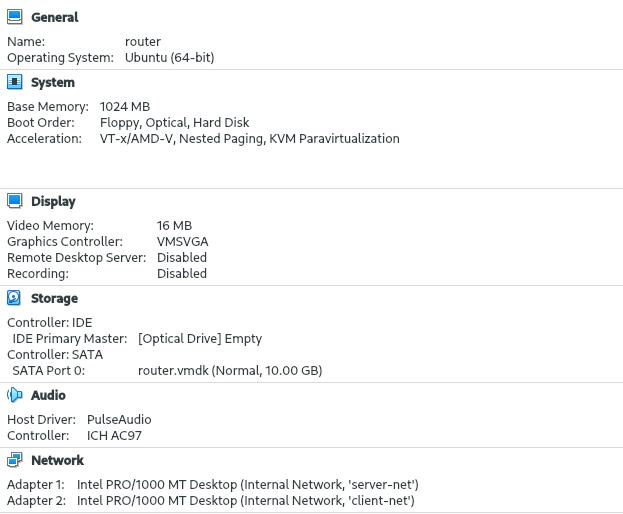
\includegraphics[scale=0.6]{figs/screenshots/router_info.png}}
   \caption{} \label{fig:router_info}
\end{figure}


\end{document}

%%
%% End of file `elsarticle-template-num.tex'.
